\subsubsection*{Installierte Schriftarten verstecken f�r Firefox}
Um die installierten Schriftarten zu verstecken, deaktiviert man in den Einstellungen die Option \textit{Webseiten das verwenden von eigenen Schriften erlauben}. Man findet die Option in den Firefox \textit{Einstellungen} auf dem Reiter \textit{Inhalt}. Klicken Sie auf den Button \textit{Erweitert}, um im folgenden Dialog Bild \ref{abb:schriftarten} die Option zu deaktivieren.\\

\begin{figure}[htb]
\begin{center}
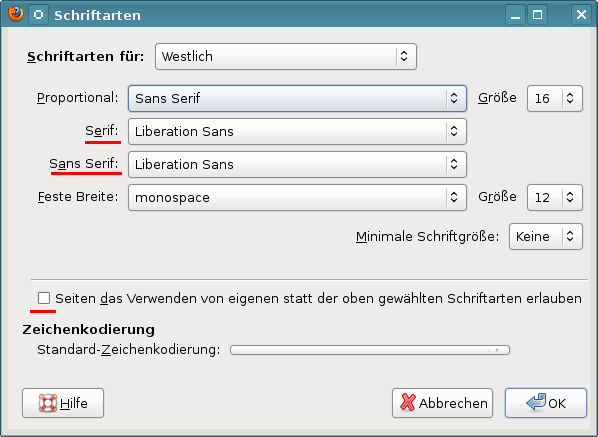
\includegraphics[scale=0.75]{../screenshots/schriftarten.png}
\caption{Schriftarten}
\label{abb:schriftarten}
\end{center}
\end{figure}

Damit kann man nur ''3'' Schriftarten auslesen. Der Browser verwendet aber auch nur die drei Standardschriften zur Darstellung der Webseiten. Damit sehen nicht alle Webseiten exakt so aus, wie es sich der Designer w�nscht. Um die Lesbarkeit zu verbessern, sollten man au�erdem gut lesbare Standardschriften verwenden. Unter Windows eignet sich \textit{Arial}, unter Linux nutzt man am besten \textit{Liberation Sans} (siehe Screenshot).


\subsubsection*{User-Agent modifizieren f�r Firefox}
Es ist nicht so einfach, den User Agent plausibel zu faken. Um durch unsachgem��e �nderung keine eindeutige Kennung zu generieren, sollte man nachdenken, bevor man etwas �ndert.\\

Man kann f�r einen Firefox nur eine andere Firefox-Kennung verwenden. Da die Browser durch individuelle Header erkennbar sind, ist eine Tarnung mit dem User-Agent eines anderen Browsers leicht als Fake zu identifizieren und man ist eindeutig identifizierbar. Einige Firefox Versionen unterscheiden sich nicht nur im User-Agent, sondern auch sehr subtil in einigen anderen HTTP-Headern. Man beachte das Leerzeichen nach dem Komma bei FF 10.0:\\
\begin{verbatim}
 ACCEPT-ENCODING "gzip,deflate"      (Firefox 3.6.x)
 ACCEPT-ENCODING "gzip, deflate"     (Firefox 10.0.x)
\end{verbatim} 

Deshalb muss man auch eine �hnliche Firefox-Version f�r den Fake nutzen, die sich in den �brigen HTTP-Headern nicht unterscheidet.Die meisten Firefox-User nutzen Windows als Betriebssystem. Daher sollte man einen Fake von Firefox f�r Windows nutzen, um in einer gr��eren Anonymt�tsgruppe abzutauchen. F�r Windows Nutzer empfehle ich keine Fakes, da man durch kleine Fehler nur eindeutiger identifizierbar wird.\\

Um die User-Agent Kennung zu �ndern, gibt man in der Adresszeile "about:config" ein und setzt die angebenen Variablen auf die Werte. Alle Werte sind vom Typ \textit{String}. Die folgenden Einstellungen des JonDoFox und TorBrowser kann man f�r Firefox 10.0.x (esr) und auch f�r Firefox 11|12|13 nutzen, wenn man einen ein eher seltenes Betriebssytem nutzt. 

\begin{center}
\begin{tabular}{ll}
Variable & Wert\\
\hline
general.useragent.override & Mozilla/5.0 (Windows NT 6.1; rv:10.0) \\
 & Gecko/20100101 Firefox/10.0\\
\hline
general.appname.override & Netscape\\
general.appversion.override & 5.0 (Windows)\\
general.oscpu.override & Windows NT 6.1\\
general.platform.override & Win32\\
general.productSub.override & 20100101\\
general.buildID.override & 0\\
general.useragent.vendor & \\
general.useragent.vendorSub & \\
\hline
\end{tabular}
\end{center}

Im Firefox 17.0 haben die Mozilla-Entwickler ein paar kleine subtile �nderungen an den gesendeten HTTP-Headern vorgenommen, so dass der Fake des Firefox 10 nicht mehr passt. Bei einem Firefox 17.0 sind folgende Werte zu setzen, um einen plausiblen Fake zu erstellen:

\begin{center}
\begin{tabular}{ll}
Variable & Wert\\
\hline
general.useragent.override & Mozilla/5.0 (Windows NT 6.1; rv:17.0)\\
 & Gecko/17.0 Firefox/17.0\\
\hline
general.appname.override & Netscape\\
general.appversion.override & 5.0 (Windows)\\
general.oscpu.override & Windows NT 6.1\\
general.platform.override & Win32\\
general.productSub.override & 20100101\\
general.buildID.override & 0\\
general.useragent.vendor & \\
general.useragent.vendorSub & \\
\hline
\end{tabular}
\end{center}

\subsubsection*{Geolocation-API deaktivieren}
Mit Hilfe der Geolocation-API kann die geografische Position des Surfer relativ genau bestimmt werden. Zur Ortsbestimmung k�nnen je nach vorhandener Hardware im Rechner die WLANs in der Umgebung genutzt werden, GPS-Hardware oder \dots Im ung�nstigsten Fall kann der Standort nur anhand der IP-Adresse bestimmt werden. Die Nutzung der Geolocation API erfolgt mit Javascript. Da man Javascript auf vielen Seiten frei�geben muss, ist eine Deaktivierung der Geolocation-API sinnvoll. Dann kann ein Webserver den Standort nur relativ ungenau anhand der IP-Adresse ermitteln.\\

Bei Firefox wird die Geoloacation API wird unter \textit{about:config} deaktiviert, indem folgende Variabale auf \textit{FALSE} gesetzt wird:

\begin{verbatim}
   geo.enabled = false
\end{verbatim} 

Diese Einstellung ist wichtig, wenn man die eigene IP-Adresse mit VPNs oder Anonymisierungsdiensten versteckt.

\subsubsection*{Kill Switch f�r Add-ons abschalten}
Die extension blocklist\footnote{ \href{http://https://addons.mozilla.org/en-US/firefox/blocked/}{https://addons.mozilla.org/en-US/firefox/blocked}} kann Mozilla nutzen, um einzelne Add-ons im Browser zu deaktivieren. Es ist praktisch ein kill switch f�r Firefox Add-ons und Plug-ins. Beim Aktualisieren der Blockliste werden detaillierte Informationen zum realen Browser und Betriebssystem an Mozilla �bertragen.

\begin{verbatim}
   https://addons.mozilla.org/blocklist/3/%7Bec8030f7-c20a
   -464f-9b0e-13a3a9e97384%7D/10.0.5/Firefox/20120608001639
   /Linux_x86-gcc3/en-US/default/Linux%202.6.37.6-smp%20
   (GTK%202.24.4)/default/default/20/20/3/
\end{verbatim}

Ich mag es nicht, wenn jemand remote irgendetwas auf meinem Rechner deaktiviert oder deaktivieren k�nnte. Unter \textit{about:config} kann man dieses Feature abschalten:
\begin{verbatim}
   extensions.blocklist.enabled = false
\end{verbatim}
